
\chapter{Advanced usage: Custom analysis}
\label{custom}

\section{Conveyor}

All offered analysis tools provided by the MGX platform are implemented as workflows
for the Conveyor\cite{CONVEYOR} workflow engine developed by B. Linke. Within Conveyor,
tools are provided as so-called ''nodes'', which resemble individual processing steps
and which are used to implement novel analysis methods by simply arranging and connecting
them into a larger workflow. Conveyor currently includes plugins providing typical
bioinformatics tools like BLAST or HMMer, but has recently been extended with dedicated
plugins aimed at metagenome analysis, like MetaCV, MetaPhyler or MetaPhlAn, which all
perform taxonomic analysis.
A dedicated Conveyor plugin provides access to MGX data structures, thereby enabling the
analysis of metagenomes stored in the MGX system with processing tools provided by Conveyor
itself.
While workflow definitions are stored in a XML-based format, a graphical user interface,
the Conveyor designer (\ref{designer}), enables users to implement new analysis by simply
placing and connecting nodes.

\begin{figure}[ht]
\centering
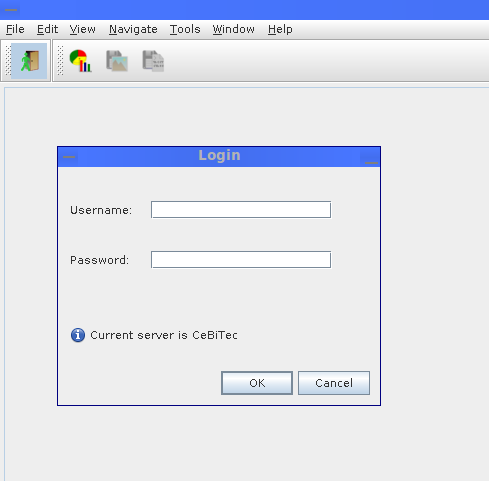
\includegraphics[width=.8\textwidth]{img/login-screen}
\caption['Conveyor Designer]{The Conveyor Designer application allows easy and user-friendly
development of custom analysis algorithms in a graphical way.}
\label{designer}
\end{figure}

As Conveyor is actively developed and new tools are continously integrated, giving a thorough
introduction is beyond the scope of this document. The most up-to-date documentation describing
Conveyor itself and the Conveyor Designer in particular can be found at the Conveyor web
site \url{http://www.uni-giessen.de/fbz/fb08/bioinformatik/software/Conveyor}.

\subsection{Getting started}

In order to implement a custom workflow, the Conveyor Designer needs to be configured
with a definition of available Conveyor plugins and node types. This is easily 
achieved by importing a plugin dump file, which contains a list of data types and
nodes provided by a Conveyor installation.

To use the Designer to implement a workflow for the MGX framework, a corresponding
plugin dump file can be obtained from within MGX by right-clicking on the 
project name.

\subsection{Workflow requirements}

In order to design custom Conveyor workflows for later usage within the MGX platform, there
are several constraints to be met which will be described in more detail.\\

First of all, a dedicated \node{GetMGXJob} node (Figure \ref{getmgxjob}) has to be present within the workflow; in addition,
this node has to be named "\textbf{mgx}". During execution of a pipeline within MGX, this node is
configured via an external configuration file, providing required information about a jobs
context, like e.g. access to a project database and associated storage.\\

\begin{figure}[ht]
\centering
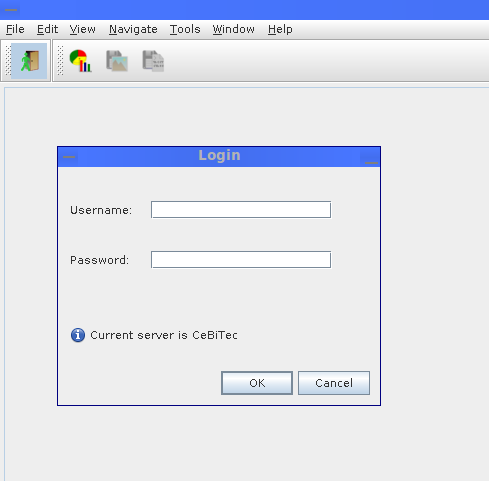
\includegraphics[width=.5\textwidth]{img/login-screen}
\caption[\node{GetMGXJob}]{The \node{GetMGXJob} node provides necessary context for executing a
workflow within MGX, such as database access. By convention, this node has to be named \textbf{mgx}.}
\label{getmgxjob}
\end{figure}

Access to metagenome DNA sequences is provided via the \node{ReadCSF} node, which will provide
all metagenome sequences for a sequencing run object within MGX, except those for which the 
``discard'' flag has been set. As pipelines are always executed
for one single analysis job, this node needs to be connected to the \node{GetMGXJob} node.\\

\begin{figure}[ht]
\centering
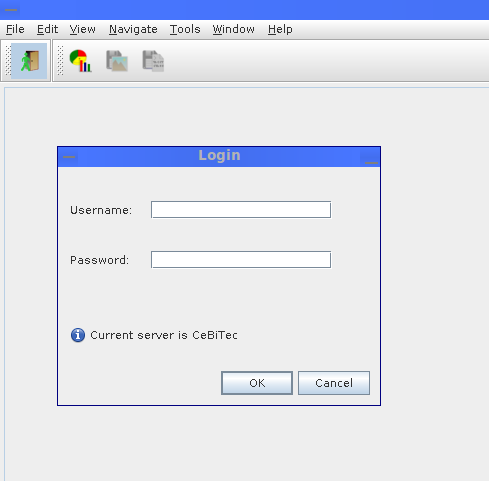
\includegraphics[width=.5\textwidth]{img/login-screen}
\caption[\node{ReadCSF}]{The \node{ReadCSF} node is used to obtained metagenome sequence data 
from within MGX; it has one input and needs to be connected to the \node{GetMGXJob} node.}
\label{readcsf}
\end{figure}

accessing sequences\\
filtering sequences\\
creating attribute types\\
annotating attributes\\
example workflow\\


